\begin{frame}{Resultados}
    \begin{table}[H]
    \centering
    \begin{tabular}{|c|c|c|c|c|} \hline
        Algortimo & Número a factorizar & IBM Device & Lanzamientos & Repeticiones \\ \hline 
        CCGN & \multirow{3}{*}{21} & - & -& \multirow{3}{*}{1000}\\  \cline{1-1} \cline{3-4}
        Shor (Local) &  & \multirow{2}{*}{Vigo}& \multirow{2}{*}{1000}& \\ \cline{1-1}
        Shor (IBM Q) &  & &  &\\\hline
    \end{tabular}
    \caption{Parámetros de entrada de cada algoritmo de factorización.}
    \label{table:parametros}
\end{table}
\end{frame}
\begin{frame}{Resultados}
    \begin{table}[H]
    \centering
    \begin{tabular}{ccc} \hline
        Algoritmo & Promedio (ms) & $\sigma$ (ms ) \\ \hline
        Clasico & 0.056 & 0.0096 \\
        Shor &0.036& 0.0153 \\
        Shor IBM &0.024 &0.0102 \\ \hline
    \end{tabular}
    \caption{Promedio y desviación estandar de cada algoritmo de factotización ejecutados en una computadora clásica y cuántica.}
    \label{tabla:resultados}
\end{table}
\end{frame}
\begin{frame}{Resultados}
    \begin{figure}[H]
    \centering
    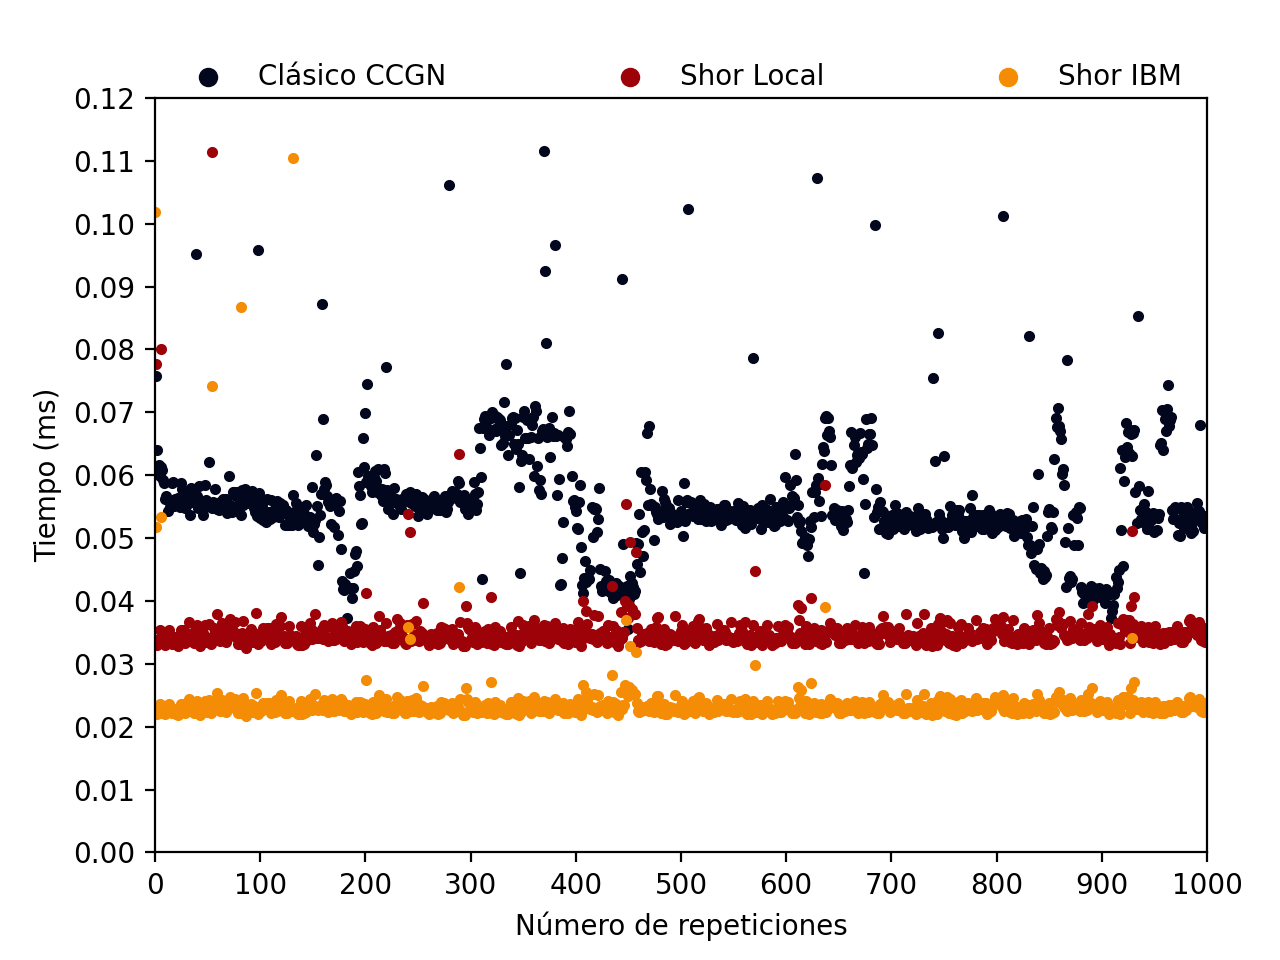
\includegraphics[scale=0.5]{images/time.png}
    \caption{Comparación de los tiempos de procesamiento de los códigos
    ejecutados en una computadora clásica y en una computadora cuántica.}
    \label{fig:time}
\end{figure}
\end{frame}